\section{Antonina Wasikowska}

Wzor na calke:\[ \int x ^ n dx= \frac{x^{n+1}}{n+1} +c\]

\vspace{5cm}
Dodane zdjecie:
\begin{figure}[htbp]
    \centering
    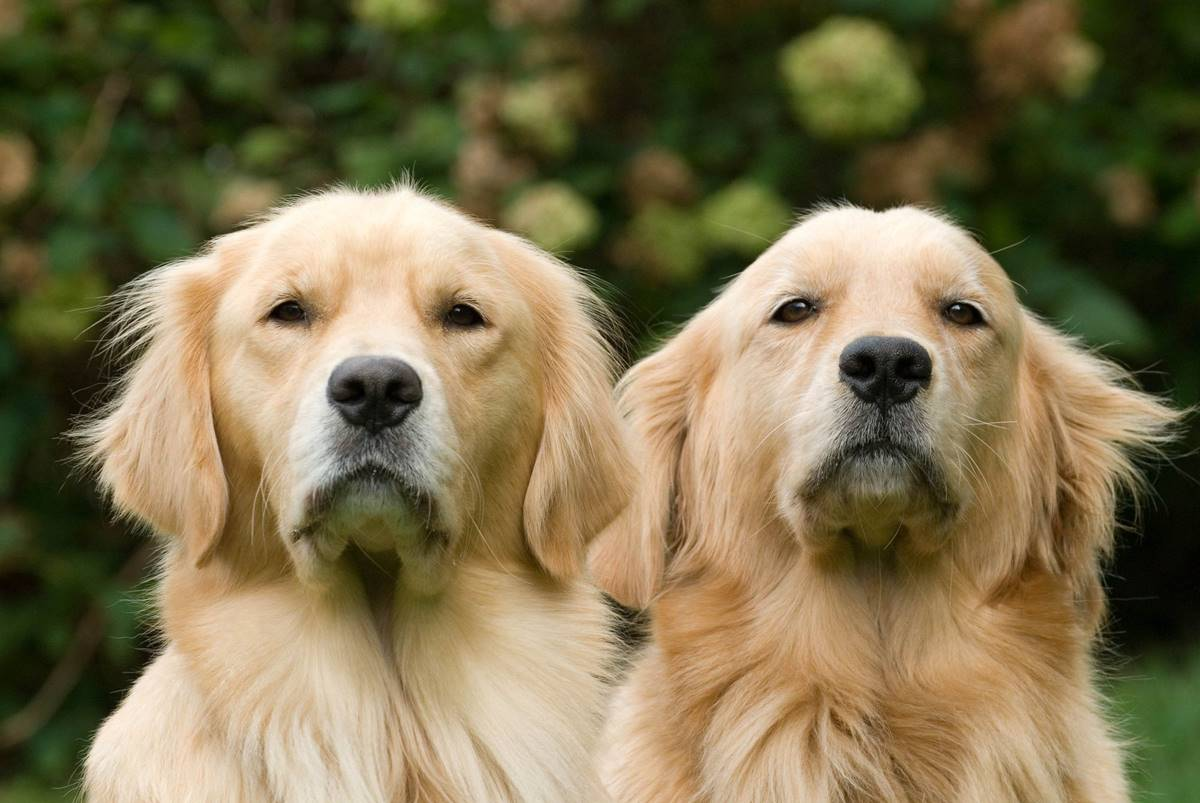
\includegraphics[width=0.9\textwidth]{pictures/dogs.png} 
    \label{fig:dogs}
\end{figure}

\vspace{1cm}

Tabela:

\input{tables/table_Antonina _Wąsikowska}
\label{}

Lista zakupów (numerowana)

\begin{enumerate}
    \item Masło
    \item Mleko
    \item Miód
    \item Kasza
\end{enumerate}

\vspace{0.5cm}


Lista rzeczy na wyjazd (nienumeowana)
\begin{itemize}
    \item Hamak
    \item Śpiwór
    \item Poduszka
\end{itemize}

\begin{flushleft}
    Trwa jesień (choć nieco zimowa). Ta \textbf{piękna, kolorowa} pora roku w Tatrach to \underline{idealny moment na wycieczki krajobrazowe}.
\end{flushleft}
\begin{center}
    \textit{Świeże powietrze i kolory zachęcają do pieszych wędrówek górskimi szlakami. Warto np. wybrać się nad Morskie Oko. Otoczenie tego jeziora jesienną porą jest urocze a szlak wiodący nad jezioro, który biegnie lasem, dostarczy jesienią wielu wrażeń wzrokowych.}
\end{center}

\vspace{1cm}
Zdjęcie psów nr :\ref{fig:dogs} przedstawia psy\par
Tabela nr \ref{fig:random} jest randomowa







